% !TEX root = ../../Diploma.tex
\section{Setup}
\subsection{Preliminary Studies in the BEM environment}
To validate the implementation of the controllers and do studies of some of the hyperparameters of the agent the BEM environment is used. The airfoil data and physical properties are taken from the NREL 5MW reference turbine \cite{jonkman_definition_2009}. The mean wind speed is $V_0=\SI{10.5}{m/s}$ and a velocity probe is placed $\SI{10.5}{m}$ upstream of the turbine.
The control variable is $M_{gen}$. The state of the environment consists of the angular velocity of the turbine and the streamwise velocity of the velocity probe. Training is conducted in six environments in parallel, with independently generated turbulent inflow. The size of the time step of the simulation is $\Delta t = \SI{0.1}{s}$.
A parameter study of the following parameters is conducted:
\begin{itemize}
	\item variance of action $\sigma_A$
	\item policy $l_2$ regularization coefficient $\varepsilon_{p,l_2}$
	\item value $l_2$ regularization coefficient $\varepsilon_{v,l_2}$
\end{itemize}
These parameters were chosen since they do not directly depend on the physics and layout of the problem. The parameters not varied are set according to \autoref{tab:params_agent}.
\begin{table}[h]
	\centering
	\caption{Parameters of agent and environment}
	\begin{tabular}{ccc}
		\toprule
		Parameter & Symbol & Value \\
		\midrule
		Time per action & $\Delta t_A$ & $\SI{1.0}{s}$ \\ 
		Number of actions per episode & $N_{A,e}$ & $500$ \\
		Number of episodes per batch & $N_{e,b}$ & $12$ \\
		Width of actor network & & $100$ \\ 
		Width of value network & & $200$ \\ 
		Variance of action & $\sigma_A$ & $0.1$ \\ 
		Importance ratio clipping & $\beta$ & $0.2$ \\ 
		Discount factor & $\gamma$ & $0.95$ \\ 
		Policy $l_2$ regularization coefficient & $\varepsilon_{p,l_2} $ & $0.1$ \\ 
		Value $l_2$ regularization coefficient & $\varepsilon_{v,l_2}$ & $0.1$ \\ 
		Value network loss coefficient & $\varepsilon_{v,l}$ & $0.5$ \\ 
		Learning rate & $\psi$ & $10^{-3}$ \\
		\bottomrule
	\end{tabular}
	\label{tab:params_agent}
\end{table}
\subsection{The LBM-ALM Environment}
\label{ssec:LBM_ALM_env}
The properties of the turbine are again taken from the NREL5 reference \cite{jonkman_definition_2009}. The diameter $D$ of the rotor is therefore $D=\SI{126}{m}$. Three turbines are placed in the center of the cross-stream plane with a distance of five diameters in streamwise direction. The first turbine is placed three diameters downstream of the inlet. The domain is $19$ diameters long and six diameters wide and high. In order to reduce computational cost, a more refined domain is placed within the first domain. It is placed in the center of the crosswise plane and one diameter downstream of the inlet. 130 velocity probes are placed in the shape of crosses upstream and between the turbines with a distance of one diameter.  The layout is shown in \autoref{fig:domain}. The inflow is turbulent with a turbulence intensity $TI$ of $5$ percent calculated as $TI = \sqrt{\frac{1}{3}(u'^2+v'^2+w'^2)}/V_0$. The parameters of the domain are gathered in \autoref{tab:params_domain}. Training of the agents is again conducted in six environments in parallel.
\begin{table}[h]
	\centering
	\caption{Parameters of the domain}
	\begin{tabular}{cc}
	\toprule
	Parameter & Value \\ 
	\midrule
	Rotor diameter & \SI{126}{m} \\ 
	Outer domain H x W x L & $\SI{6}{D} \times \SI{6}{D} \times \SI{19}{D}$ \\ 
	Outer domain resolution & $\SI{8}{nodes/D}$ \\ 
	Inner domain H x W x L & $\SI{5}{D} \times \SI{5}{D} \times \SI{16}{D}$ \\ 
	Inner domain resolution & $\SI{16}{nodes/D}$ \\ 
	Turbulence intensity & $\SI{5}{\percent} $ \\ 
	Mean wind speed & $\SI{10.5}{m/s} $ \\
	\bottomrule
	\end{tabular}
	\label{tab:params_domain}
\end{table}
\begin{figure}
	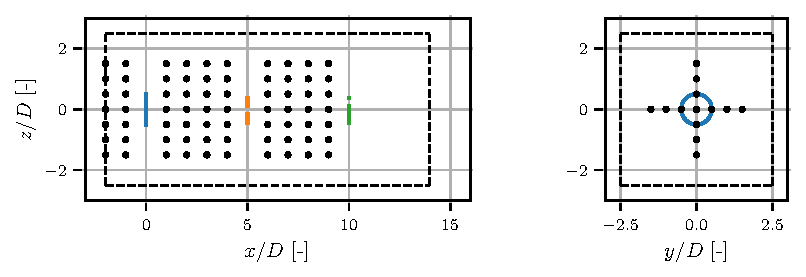
\includegraphics{diagrams/domain.pdf}
	\caption{Layout of the computational domain in the LBM-ALM environment. $\bullet$ Velocity probes \\ \legendThree{Turbine 0}{Turbine 1}{Turbine 2} \rule[3pt]{3pt}{1pt}\hspace{1pt}\rule[3pt]{3pt}{1pt}\hspace{1pt}\rule[3pt]{3pt}{1pt}\hspace{1pt}\rule[3pt]{3pt}{1pt} Inner domain \rule[3pt]{15pt}{1pt} Outer domain. }
	\label{fig:domain}
\end{figure}

\subsection{Optimizing Specific Behaviour}
\label{ssec:dyn_description}
In the LBM-ALM Environment with the domain as specified in \autoref{ssec:LBM_ALM_env}, an agent controlling the amplitude of a sinusoidal variation of the pitch angles according to the helix strategy will be trained. Therefore the equation described in \eqref{control_amplitude} will be modified like this:
\begin{equation}
	\varphi(t) = \varphi_{base} + \sum^{N_a}_{i=0} A_{\varphi,i} \cos(2 \pi f_{\phi,i} t + \Psi + \Psi_0)
\end{equation}
$\Psi_0$ is the initial offset of the blade. The frequency $f_{\Phi,0}$ is chosen according to Frederik et al. so that the Strouhal Number $\mathrm{St} = f_{\Phi, 0} D/V_0 = 0.25$. In difference to the setup by Frederik et al., the angular velocity of the rotor will not be constant, but is determined by \eqref{eq:ang_mom}. The generator torque is controlled by a greedy controller. Two different configurations of the agent will be compared. The first agent has ten nodes per layer and the state of the environment includes angular velocity and azimuth, while the second agent has $400$ nodes per layer and the state additionally includes the streamwise velocity of the velocity probes. The other parameters of both of the agents are the same as in \autoref{tab:params_agent}.
\subsection{Learning New Behaviour}
\label{ssec:new_behaviour_description}
To assess whether the RL agent is able to discover a new control strategy for wind farm control, an agent controlling the generator torque is tested, again in the environment specified by \autoref{ssec:LBM_ALM_env}. Three different agents will be compared. The first agent has a discount rate of $\gamma = 0.95$ and a number of actions per episode $N_{A,e} = 500$, which corresponds to setup used in the preliminary studies. The second agent has the same $N_{A,e}$ but a discount rate of $\gamma = 0.99$. The third agent also has a discount rate of $\gamma = 0.99$ but the number of actions per episode is $N_{A,e} = 1500$. The parameters differing from \autoref{tab:params_agent} are gathered in \autoref{tab:params_new_b}. 
\begin{table}[h]
	\centering
	\caption{Parameters of agent for learning new behaviour}
	\begin{tabular}{cccc}
		\toprule 
		Parameter & Case 1 & Case 2 & Case 3 \\ 
		\midrule
		$\gamma$ & $0.95$ & $0.99$ & $0.99$ \\ 
		$N_{A,e}$ & $500$ & $500$ & $1500$ \\ 
		Width of actor network & $400$ & $400$ & $400$ \\
		\bottomrule
	\end{tabular}
	\label{tab:params_new_b}
\end{table}\\
This choice of parameters is motivated by a closer look at the meaning of reward and return in the context of this setup. The number of actions in the time it takes for information to travel from the first turbine to the second turbine can be estimated to be $N_{t,T} = d_T/(v_0 \cdot \Delta t_A) = 60$. This is a lower bound on the estimate, since information might travel slower due to a reduced velocity in the wake. The reward is calculated as follows: 
\begin{equation} 
\mathsf{R}(t) = \frac{P_0(t) + P_1(t) + P_2(t)}{\SI{}{MW}}.
\end{equation} Combining this with \eqref{eq:return}, the return of an action at the first turbine should be calculated like this:
\begin{equation}
	\mathsf{G}_{t,0} = \sum^\mathsf{T}_{t'=t} \sum_{i=0}^{N_T-1}P_i(t'+iN_{t,T})\gamma^{t'+iN_{t,T}-t}.
\end{equation}
Considering the values of this setup, a discount rate of $0.95$ leads to a static discount of the seconds turbine power of around $95$ percent, whereas a discount rate of $0.99$ discounts the power of the second turbine only by $45$ percent. When trying to achieve a combined control a high discount rate therefore seems to be beneficial. However, this also leads to little discounting of the power after information of the first turbine has reached the second turbine and therefore makes the return more noisy, as information that is probably less influenced by the action of the first turbine is added to the return. Therefore a balance between these two influences has to be found.


